\begin{tiny}(Cpb17)\end{tiny} Notons $D_n$ l'événement \og la Douche fonctionne au jour $n$\fg~ et $\overline{D_n}$ l'événement contraire. Ils forment un système complet. L'énoncé se traduit simplement par
\[
  \p_{D_n}(D_{n+1}) = f, \hspace{0.5cm} \p_{\overline{D_n}}(D_{n+1}) = v.
\]
Notons $p_n = \p(D_n)$. La suite vérifie une relation de récurrence à cause de la formule des probabilités totales:
\[
  p_{n+1} = f p_n + v(1-p_n)
  = (f-v)p_n + v.
\]
Notons $q$ le point fixe
\[
  q = (f-v)q+v 
  \Rightarrow
  q = \frac{v}{v + 1 -f}.
\]
On en déduit
\[
  p_n = q + (f-v)^n(1-q).
\]
Notons que $0 < q <1$ et $-1< -v < f-v < f <1$ car $f$ et $v$ sont dans $]0,1[$.\newline
La suite $q_n$ converge donc vers $q$.\newline
La configuration satisfaisante correspond à $q \geq 0.9$
\[
  q \geq 0.9 \Leftrightarrow v \geq 0.9(v+1-f)
  \Leftrightarrow 0.9 f + 0.1v \geq 0.9.
\]
\begin{figure}[h!]
  \centering
  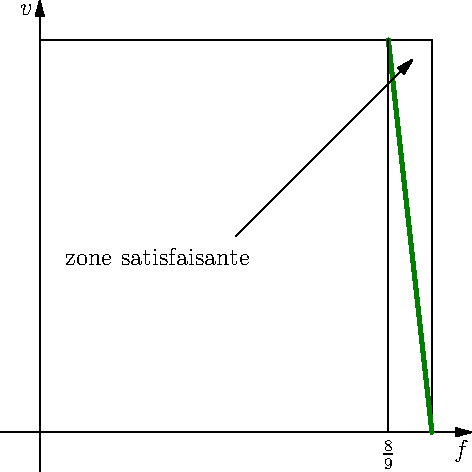
\includegraphics[width=4cm]{Cpb17_1.pdf}
  % Cpb17_1.pdf: 198x198 px, 72dpi, 6.99x6.99 cm, bb=0 0 198 198
\end{figure}
